\section{Results}
\subsection{Primary frozen synthetic holdout}
Table~\ref{tab:primary} and Figure~\ref{fig:primary} show the paired comparison on exactly the same 15 queues. The candidate recovered 18 additional expert top-20 incidents and recalled 10 additional incidents in the first 20 groups. P@10 rose by six credited positions. These are absolute differences of 6.00, 3.33, and 4.00 percentage points, respectively; no statistical significance claim is made.
\begin{table}[ht]\centering\small\caption{Frozen paired holdout results. Fractions use evaluator opportunity denominators. Differences are candidate minus baseline; percentage differences are percentage points.}\label{tab:primary}\begin{tabularx}{\linewidth}{@{}Yrrr@{}}\toprule Metric & Frozen baseline & Endpoint fallback & Difference\\\midrule Incident Recall@20 & 250/300 (83.33\%) & 260/300 (86.67\%) & +10 (+3.33 pp)\\ Group recoverability & 263/300 (87.67\%) & 281/300 (93.67\%) & +18 (+6.00 pp)\\ P@10 & 107/150 (71.33\%) & 113/150 (75.33\%) & +6 (+4.00 pp)\\ Grouped-pair precision & 19,459/19,459 (100\%) & 20,117/20,117 (100\%) & 0 pp\\ False grouped pairs & 0 & 0 & 0\\ Mixed groups & 0 & 0 & 0\\\bottomrule\end{tabularx}\end{table}
\begin{figure}[ht]\centering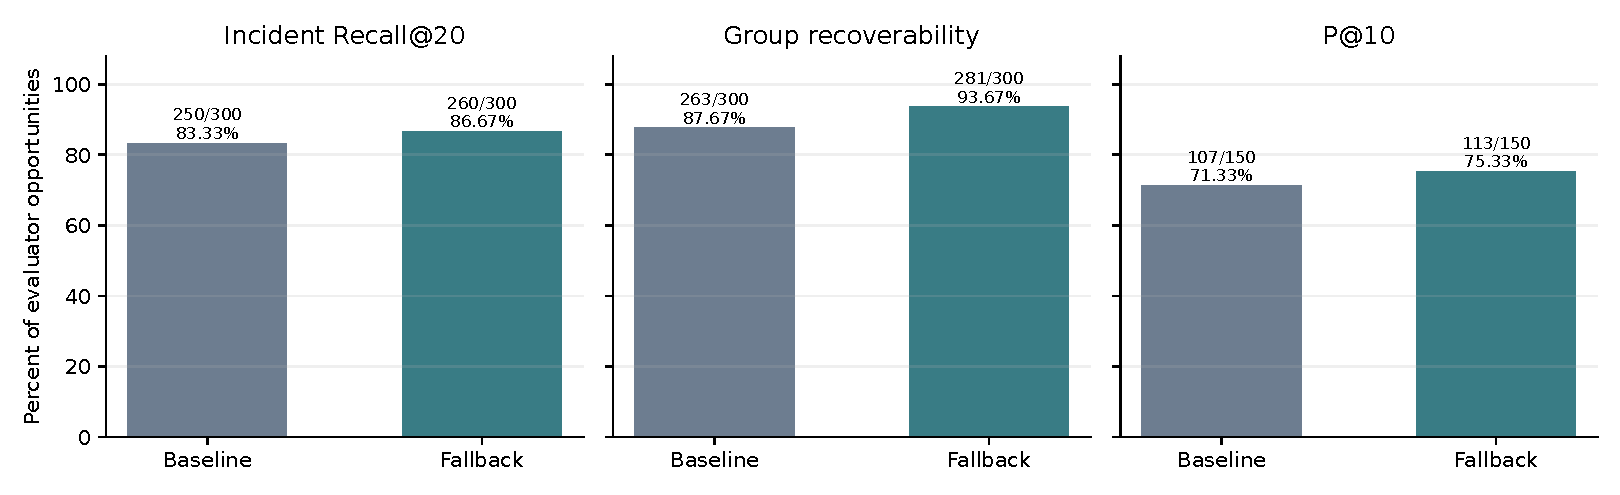
\includegraphics[width=\linewidth]{figures/phase33_results.pdf}\caption{Frozen synthetic holdout metrics generated directly from the verified holdout summary, with exact counts and evaluator denominators. Axes run from zero to allow direct comparison; the three panels represent different evaluation opportunities and must not be added together.}\label{fig:primary}\end{figure}

The simulator-truth audit classified all 28 newly accepted fallback unions and all 711 total candidate accepted unions as genuine. It recorded 150 false relationship-token rejections and 35 genuine-token abstentions. These token counts refer to a different evaluation unit than pair precision. Figure~\ref{fig:safety} displays the all-group safety results; all 15 queues had zero false pairs and zero mixed groups in both arms. Queue-level Recall@20 nevertheless fell by one incident in two queues, and P@10 fell in two queues. Aggregate gains therefore do not imply uniform queue gains.
\begin{figure}[ht]\centering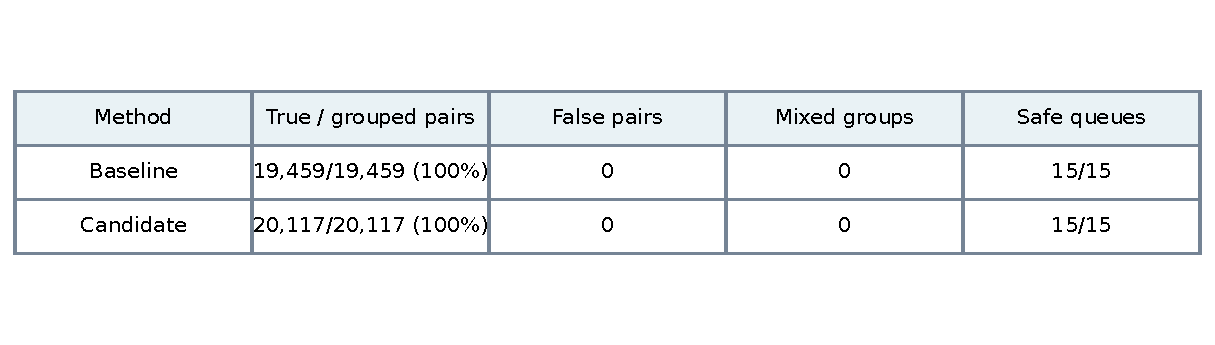
\includegraphics[width=.9\linewidth]{figures/safety_results.pdf}\caption{Grouped-pair and mixed-group outcomes on the 15-queue controlled holdout. Pair precision uses all within-group pairs; the count of safe queues is based on zero false grouped pairs and zero mixed groups in each queue. Zero observed errors under simulator truth is not a bound on real-world error rates.}\label{fig:safety}\end{figure}

\subsection{Development-only and historical evidence}
Table~\ref{tab:development} summarizes separate ranking and evidence studies. Later development scores are not substituted for the frozen holdout or construed as a performance trajectory. The earlier historical synthetic holdout had 407/600 Recall@20 and 451/600 recoverability on another population; its scores are not directly comparable. An unsafe richer-claim development configuration produced 2,580 false pairs and 22 mixed groups, whereas independent-claim verification on that development cohort preserved zero false pairs and recovered 166/200 incidents.
\begin{table}[ht]\centering\small\caption{Later investigations on distinct development-only cohorts. B and C are matched within each row; they are not comparable across rows as successive improvements.}\label{tab:development}\begin{tabularx}{\linewidth}{@{}p{29mm}Yrrr@{}}\toprule Study & Question & Baseline R@20 & Candidate R@20 & Candidate recoverability\\\midrule Ranking feature study & Post-group score & 264/300 & 267/300 & 277/300\\ Near-boundary rank study & Reorder below first ten & 258/300 & 258/300 & 273/300\\ Evidence-aware rank study & Visible evidence features & 265/300 & 262/300 & 277/300\\ Evidence availability & Frozen condition, stress tests & 257/300 & --- & 267/300\\ Hard-negative rank study & Pairwise trained reordering & 263/300 & 262/300 & 279/300\\\bottomrule\end{tabularx}\end{table}
